\documentclass[a4paper,12pt]{article}
% -------------------------------------------------------------------
%                  Essential packages (used in template)
% -------------------------------------------------------------------

\usepackage[utf8]{inputenc}                   % Allow Umlauts (ä, ö, ü)
\usepackage[ngerman]{babel, translator}       % German LaTeX-intern descriptors (Abbildungen, ...)
\usepackage{mathptmx}                         % Font "Times New Roman" in mathematical Environments
\usepackage{courier}                          % Support the use of font "Courier" (used in listings)
\usepackage[T1]{fontenc}                      % Change LaTeX font encoding to support modern fonts
\usepackage{fix-cm}                           % Fix sizes at which CM and EC fonts can be used

\usepackage{geometry}                         % Change text bounds on a per-page basis
\usepackage{fancyhdr}                         % Allow easy customization of headers and footers

\usepackage[ddmmyyyy]{datetime}               % Reformat times from LaTeX commands like \today

\usepackage[dvipsnames]{xcolor}               % Support text colorization

\usepackage{colortbl}                         % Support applying colors to tables
\usepackage{array}                            % Tables with fixed column size
\usepackage{longtable}                        % Support multi-page tables
\usepackage{multicol}                         % Additional settings for \multicolumn
\usepackage{multirow}                         % Additional settings for \multirow

\usepackage[hyphens,obeyspaces,spaces]{url}   % Allow urls to have line breaks at "-"
\usepackage{microtype}                        % Enable "Blocksatz"

\usepackage{float}                            % Support for table H option
\usepackage{floatflt}                         % Support text wrapping around floating environments
\usepackage{wrapfig}                          % Support text wrapping around figures

\usepackage{graphicx}                         % Support including graphics environments for images
\usepackage{caption}                          % Provide greater customization around captions
\usepackage{subcaption}                       % Caption support for subfigures
\usepackage{pdfpages}                         % Include existing PDFs into the work

\usepackage[onehalfspacing]{setspace}         % Set line spacing to be 1.5x the default
\usepackage{listings}                         % Code block support for LaTeX

\usepackage[titles]{tocloft}                  % More options to modify list of figures & tables
\usepackage{nomencl}                          % Support for nomenclatures ("Symbolverzeichnis")

\usepackage{amsmath}                          % Includes a plethora of mathematical packages 
\usepackage{amssymb}                          % Source mathematical symbols like \sin
\usepackage{amsthm}                           % Better theorems
\usepackage{upgreek}                          % Use \Upomega to get a straight \Omega
\usepackage{siunitx}                          % Unified support for si units

\usepackage{ifthen}                           % Support better if statements in LaTeX
\usepackage{etoolbox}                         % Easily patch commands

\usepackage{hyperref}                         % Clickable hyperlinks in Table of Contents

% Support list of acronyms and glossary
\usepackage[
  toc,
  nogroupskip,
  nonumberlist,
  nopostdot,
  acronyms,
  shortcuts,
  translate=babel
]{glossaries}

% Track the total count of different environments
% Needs to be imported because LaTeX resets these counter on a chapter basis
\usepackage[figure,table,lstlisting,xspace]{totalcount}

% Annotate different information directly into the document
\setlength{\marginparwidth}{2cm}
\usepackage[
  colorinlistoftodos,
  prependcaption,
  textsize=tiny
]{todonotes}

% -------------------------------------------------------------------
%                 Useful packages (not used in template)
% -------------------------------------------------------------------

% Create electrical diagrams from within LaTeX
\usepackage[
  european,
  oldvoltagedirection,
  straightvoltages,
  siunitx
]{circuitikz}

% Annotate images with standard tikz macros
\usepackage{tikz-imagelabels}

% page margins
\geometry{
  left=2.5cm,
  right=2.5cm,
  top=2.5cm,
  bottom=3cm
}

% Disable single lines at the start of a paragraph (Schusterjungen)
\clubpenalty=10000

% Disable single lines at the end of a paragraph (Hurenkinder)
\widowpenalty=10000
\displaywidowpenalty=10000

% Fixed size table columns
\newcolumntype{L}[1]{>{\raggedright\arraybackslash}p{#1}}
\newcolumntype{C}[1]{>{\centering\arraybackslash}p{#1}}
\newcolumntype{R}[1]{>{\raggedleft\arraybackslash}p{#1}}

\renewcommand{\arraystretch}{1.2}                       % Distance between lines in tables

\captionsetup{justification=raggedright}                % Align captions to the left

\setcounter{secnumdepth}{3}                             % Only allow nesting 3 layers (down to subsubsections)

% Set convention to german (comma instead of point delimiter for floats)
\sisetup{locale = DE}

% -------------------------------------------------------------------
%                     Usability & visual changes
% -------------------------------------------------------------------

% Create a better looking header and footer
\pagestyle{fancy}
\fancyhf{}
\lhead{\nouppercase{\leftmark}}
\rfoot{\thepage}

% Automatically generate a box around figure environments
\floatstyle{boxed}
\restylefloat{figure}

% Set toc sections to be clickable
\hypersetup{
  colorlinks,
  citecolor=black,
  filecolor=black,
  linkcolor=black
}

\frenchspacing                                          % Insert one space after a sentence, not 2

\renewcommand{\UrlFont}{\color{blue}\rmfamily\itshape}  % URLs should be displayed in blue
\renewcommand{\dateseparator}{.}                        % Dates are written like 01.01.1970, not 01-01-1970
\renewcommand{\nomname}{Symbolverzeichnis}              % Nomenclature in german is "Symbolverzeichnis"

\addto{\captionsngerman}{
  \renewcommand*{\figurename}{Abb.}                     % Figures should be displayed as "Abb. x"
  \renewcommand*{\tablename}{Tab.}                      % Tables should be displayed as "Tab. x"
  \renewcommand*{\lstlistingname}{Code}                 % Code should be displayed as "Code x"
}

% -------------------------------------------------------------------
%                        Code listing setup
% -------------------------------------------------------------------

\lstset{
  basicstyle=\small\ttfamily\color{black},      % Font size used for the code
  commentstyle=\ttfamily\color{gray},           % Comment style
  keywordstyle=\ttfamily\color{blue},           % Keyword style
  stringstyle=\color{ForestGreen!30!LimeGreen}, % String literal style
  frame=single,                                 % Add a frame around the code
  showstringspaces=false,                       % Don't underline spaces within strings only
  captionpos=b,                                 % Set caption-position to bottom
  backgroundcolor=\color{white},                % Background color
}

% To style lstlistlisting like the lof, you first have to register it
% to tocloft, as mentioned in https://tex.stackexchange.com/a/27648/27635
\makeatletter
\begingroup\let\newcounter\@gobble\let\setcounter\@gobbletwo
  \globaldefs\@ne \let\c@loldepth\@ne
  \newlistof{listings}{lol}{\lstlistlistingname}
\endgroup
\let\l@lstlisting\l@listings
\makeatother

% -------------------------------------------------------------------
%                         Redefining geometry
% -------------------------------------------------------------------

% Figures
\renewcommand{\cftfigpresnum}{Abb.~}
\renewcommand{\cftfigaftersnum}{:}
\setlength{\cftfignumwidth}{2cm}
\setlength{\cftfigindent}{0cm}

% Tables
\renewcommand{\cfttabpresnum}{Tab.~}
\renewcommand{\cfttabaftersnum}{:}
\setlength{\cfttabnumwidth}{2cm}
\setlength{\cfttabindent}{0cm}

% Listings
\renewcommand*{\cftlistingspresnum}{\lstlistingname~}
\renewcommand*{\cftlistingsaftersnum}{:}
\settowidth{\cftlistingsnumwidth}{\cftlistingspresnum}
\addtolength{\cftlistingsnumwidth}{1cm}
\setlength{\cftlistingsindent}{0cm}

\setlength{\parindent}{0cm}                             % Don't indent start of paragraph
\setlength{\parskip}{6pt}                               % Lines are seperated by 6pt

\setlength{\headheight}{1.25cm}
\setlength{\footskip}{1cm}
\setlength{\headsep}{1cm}

% -------------------------------------------------------------------
%                    Custom counters & commands
% -------------------------------------------------------------------

\newcounter{countacronym}
\DeclareTotalCounter{countacronym}
\newcommand*{\acr}[1]{\acrshort{#1}\stepcounter{countacronym}}
\newcommand*{\Acr}[1]{\acrlong{#1}\stepcounter{countacronym}}

\newcounter{countnomen}
\DeclareTotalCounter{countnomen}
\newcommand*{\nomen}[2]{\nomenclature{#1}{#2}\stepcounter{countnomen}}
\newcommand{\nomunit}[1]{\renewcommand{\nomentryend}{\hspace*{\fill}#1}}
\newcommand{\nomsi}[1]{\nomunit{[\si{#1}]}}

% NOTE: Don't use glossary references in section names
\newcounter{countglossary}
\DeclareTotalCounter{countglossary}
\let\oldGls\Gls
\let\oldgls\gls
\let\oldGlspl\Glspl
\let\oldglspl\glspl
\renewcommand*{\Gls}[1]{\oldGls{#1}\stepcounter{countglossary}}
\renewcommand*{\Glspl}[1]{\oldGlspl{#1}\stepcounter{countglossary}}
\renewcommand*{\gls}[1]{\oldgls{#1}\stepcounter{countglossary}}
\renewcommand*{\glspl}[1]{\oldglspl{#1}\stepcounter{countglossary}}

% TODO annotations
\newcounter{counttodo}
\DeclareTotalCounter{counttodo}
\newcommand{\note}[2][]{
  \todo[color=green!25,bordercolor=green,tickmarkheight=3pt,#1]{#2}
  \stepcounter{counttodo}
}
\newcommand{\unsure}[2][]{
  \todo[color=Plum!25,bordercolor=Plum,tickmarkheight=3pt,#1]{#2}
  \stepcounter{counttodo}
}
\newcommand{\change}[2][]{
  \todo[color=blue!25,bordercolor=blue,tickmarkheight=3pt,#1]{#2}
  \stepcounter{counttodo}
}

\newcommand{\imgref}[1]{\hyperref[#1]{Abbildung~\getrefnumber{#1}}}
\newcommand{\tabref}[1]{\hyperref[#1]{Tabelle~\getrefnumber{#1}}}
\newcommand{\coderef}[1]{\hyperref[#1]{Code~\getrefnumber{#1}}}
\newcommand{\mathref}[1]{\hyperref[#1]{Gleichung~\getrefnumber{#1}}}
\newcommand{\secref}[1]{\hyperref[#1]{Abschnitt~\getrefnumber{#1}}}

% Preload custom user settings & packages
\IfFileExists{./Custom.tex}{\include{Custom}}{}

% ===========================================================================
%           Wrap document environment with HSCDocument environment
% ===========================================================================

\AddToHook{env/HSCDocument/before}{

  % Register different entries: glossary, nomenclature, acronyms
  \makeglossaries
  \hyphenation{
  An-triebs-strän-ge
}
  \newacronym{FEIF}{FEIF}{Fakultät Elektrotechnik und Informationstechnik}
\newacronym{WYSIWYG}{WYSIWYG}{What You See Is What You Get}
\newacronym{EBA}{EBA}{exemplarische Beispielabkürzung}
  \makenomenclature
  \nomenclature[01]{\textbf{Symbol}}{\textbf{Bedeutung} \nomunit{\textbf{[phys. Einheit]}}}

\nomen{$i$}{ganzzahlige Laufvariable}
\nomen{$n$}{Umfang der Messreihe oder Stichprobe}
\nomen{$s$}{empirische Standardabweichung \nomsi{\metre}}
\nomen{$\overline{x}$}{Mittelwert der Stichprobe \nomsi{\metre}}
\nomen{$x_i$}{Einzelmesswert \nomsi{\metre}}
  \newglossaryentry{Glossar}
{
    name=Glossar,
    plural=Glossare,
    description={"selbstständig oder als Anhang eines bestimmten Textes erscheinendes Wörterverzeichnis" \cite{Duden}}
}

  \begin{document}
}

\AddToHook{env/HSCDocument/after}{
  \end{document}
}

\makeatletter
\define@key{HSCDocument@keys}{preset}{\def\DocumentType{#1}}
\makeatother

\newenvironment{HSCDocument}[1][]{

  \makeatletter
  \setkeys{HSCDocument@keys}{
    preset=Custom,
    #1
  }
  \makeatother

  % Don't display "a as ä etc.
  \shorthandoff{"}

  % ===========================================================================
  %                             Document header
  % ===========================================================================

  \newgeometry{
    left=2.5cm,
    right=2.5cm,
    top=2.5cm,
    bottom=2.5cm
  }

  \begin{titlepage}
    \ifthenelse{\equal{\DocumentType}{Praxisbericht}}
      {\selectlanguage{ngerman}
\centering
% \includesvg[inkscapelatex=false,width=.8\textwidth]{framework/Logo_HS_Coburg.svg}

\includegraphics[width=.8\textwidth]{framework/Logo_HS_Coburg}

\begin{Large}
  Hochschule für angewandte Wissenschaften Coburg\\
  Fakultät Elektrotechnik und Informatik\par
\end{Large}
\vspace{1.5cm}

\Large{Studiengang: \Studiengang}
\vspace{1.5cm}

\Large{Praxisbericht}
\vspace{1cm}

\huge{\Autorenname}
\vspace{1.5cm}

\begin{table}[H]
  \begin{tabular}{|L{3cm}|L{11cm}|}
  \hline
  Unternehmen & \Unternehmen        \\
              & \Abteilung          \\
              & \Strasse            \\
              & \Ort                \\
  \hline
  Zeitraum    & \Beginn \ bis \Ende \\
  \hline
  \end{tabular}
\end{table}

\large{Abgabe des Berichts: \Abgabe}

\begin{table}[H]
  \begin{tabular}{|L{3cm}|L{6cm}|L{5cm}|}
    \multicolumn{3}{l}{Freigabe zur Vorlage des Praxisberichts an der HS Coburg:} \\
    \hline
    Betreuer & \Betreuer & \\
    \hline
    Funktion & \Funktion & \textbf{\textit{Ort, Datum}}\\
    \hline
    Telefon & \Telefon & \\
    \cline{1-2}
    Email & \Email & \\
    \hline
    & & \textbf{\textit{Unterschrift Betreuer}}\\
    \hline
  \end{tabular}
\end{table}
}
      {
        \ifthenelse{\equal{\DocumentType}{Bachelorarbeit}}
          {\centering

\includegraphics[width=.8\textwidth]{framework/Logo_HS_Coburg}

\begin{Large}
  Hochschule für angewandte Wissenschaften Coburg\\
  Fakultät Elektrotechnik und Informatik\par
\end{Large}
\vspace{1.5cm}

\Large{Studiengang: \Studiengang}
\vspace{1.5cm}

\Large{\DocumentType}
\vspace{1cm}

\Huge{\Titel}
\vspace{2cm}

\huge{\Autorenname}
\vspace{2cm}

\Large{Abgabe der Arbeit: \Abgabe}

\Large{Betreut durch:}

\Large{\Dozent, Hochschule Coburg}
}
          {
            \ifthenelse{\equal{\DocumentType}{Masterarbeit}}
              {\centering

\includegraphics[width=.8\textwidth]{framework/Logo_HS_Coburg}

\begin{Large}
  Hochschule für angewandte Wissenschaften Coburg\\
  Fakultät Elektrotechnik und Informatik\par
\end{Large}
\vspace{1.5cm}

\Large{Studiengang: \Studiengang}
\vspace{1.5cm}

\Large{\DocumentType}
\vspace{1cm}

\Huge{\Titel}
\vspace{2cm}

\huge{\Autorenname}
\vspace{2cm}

\Large{Abgabe der Arbeit: \Abgabe}

\Large{Betreut durch:}

\Large{\Dozent, Hochschule Coburg}
}
              {
                \IfFileExists{./CustomHeader.tex}{
                  \include{CustomHeader}
                }{
                  ERROR: Please use one of the following values as parameter
                  to the HSCdocument environment:\\
                  "Praxisbericht", "Bachelorarbeit", "Masterarbeit"\\

                  To create your own document header, just create a file
                  "CustomHeader.tex" in the document root.
                }
              }
          }
      }
  \end{titlepage}

  \restoregeometry

  % Header is considered the 1st page
  \addtocounter{page}{1}

  % ===========================================================================
  %                              Page Ordering
  % ===========================================================================

  % Set image path to "Bilder" subdirectory
  \graphicspath{{Bilder/}}

  % Optional notice to the reader ("Vermerk")
  \IfFileExists{./Sektionen/Vermerk.tex}{
    \newpage
    \thispagestyle{empty}
    \include{Sektionen/Vermerk}
  }{}

  % Abstract
  \IfFileExists{./Sektionen/Abstract.tex}{
    \newpage
    \fancypagestyle{abstract}{
      \fancyhead[L]{Abstract}
    }
    \thispagestyle{abstract}
    \include{Sektionen/Abstract}
  }{}

  \newpage
  \tableofcontents

  \iftotalfigures
    \newpage
    \phantomsection
    \addcontentsline{toc}{section}{\listfigurename}
    \listoffigures
  \fi

  \iftotaltables
    \newpage
    \phantomsection
    \addcontentsline{toc}{section}{\listtablename}
    \listoftables
  \fi

  \iftotallstlistings
    \newpage
    \phantomsection
    \addcontentsline{toc}{section}{\lstlistlistingname}
    \lstlistoflistings
  \fi

  % Nomenclature ("Symbolverzeichnis")
  \iftotalcountnomens
    \newpage
    \phantomsection
    \addcontentsline{toc}{section}{\nomname}
    \printnomenclature[1in]
  \fi

  % Acronyms
  \iftotalcountacronyms
    \newpage
    \setglossarystyle{super}
    \printglossary[type=\acronymtype]
  \fi

  \newpage
}
{
  % Bibliography
  \iftotalcountcitations
    \newpage
    \phantomsection
    \addcontentsline{toc}{section}{\refname}
    \printbibliography
  \fi

  % Glossary
  \iftotalcountglossarys
    \newpage
    \setglossarystyle{altlist}
    \printglossary
  \fi

  % Appendix
  \IfFileExists{./Sektionen/Anhang.tex}{
    \newpage
    \appendix
    \renewcommand{\thesection}{A\arabic{section}}
    \section{Anhang}

Ist die Datei "Anhang.tex" vorhanden, so wird diese automatisch am Ende des Dokuments eingebunden.
  }{}

  % Declaration of Honor
  \newpage
  \phantomsection
  \addcontentsline{toc}{section}{\declarationname}
  \lhead{\declarationname}
  \thispagestyle{empty}

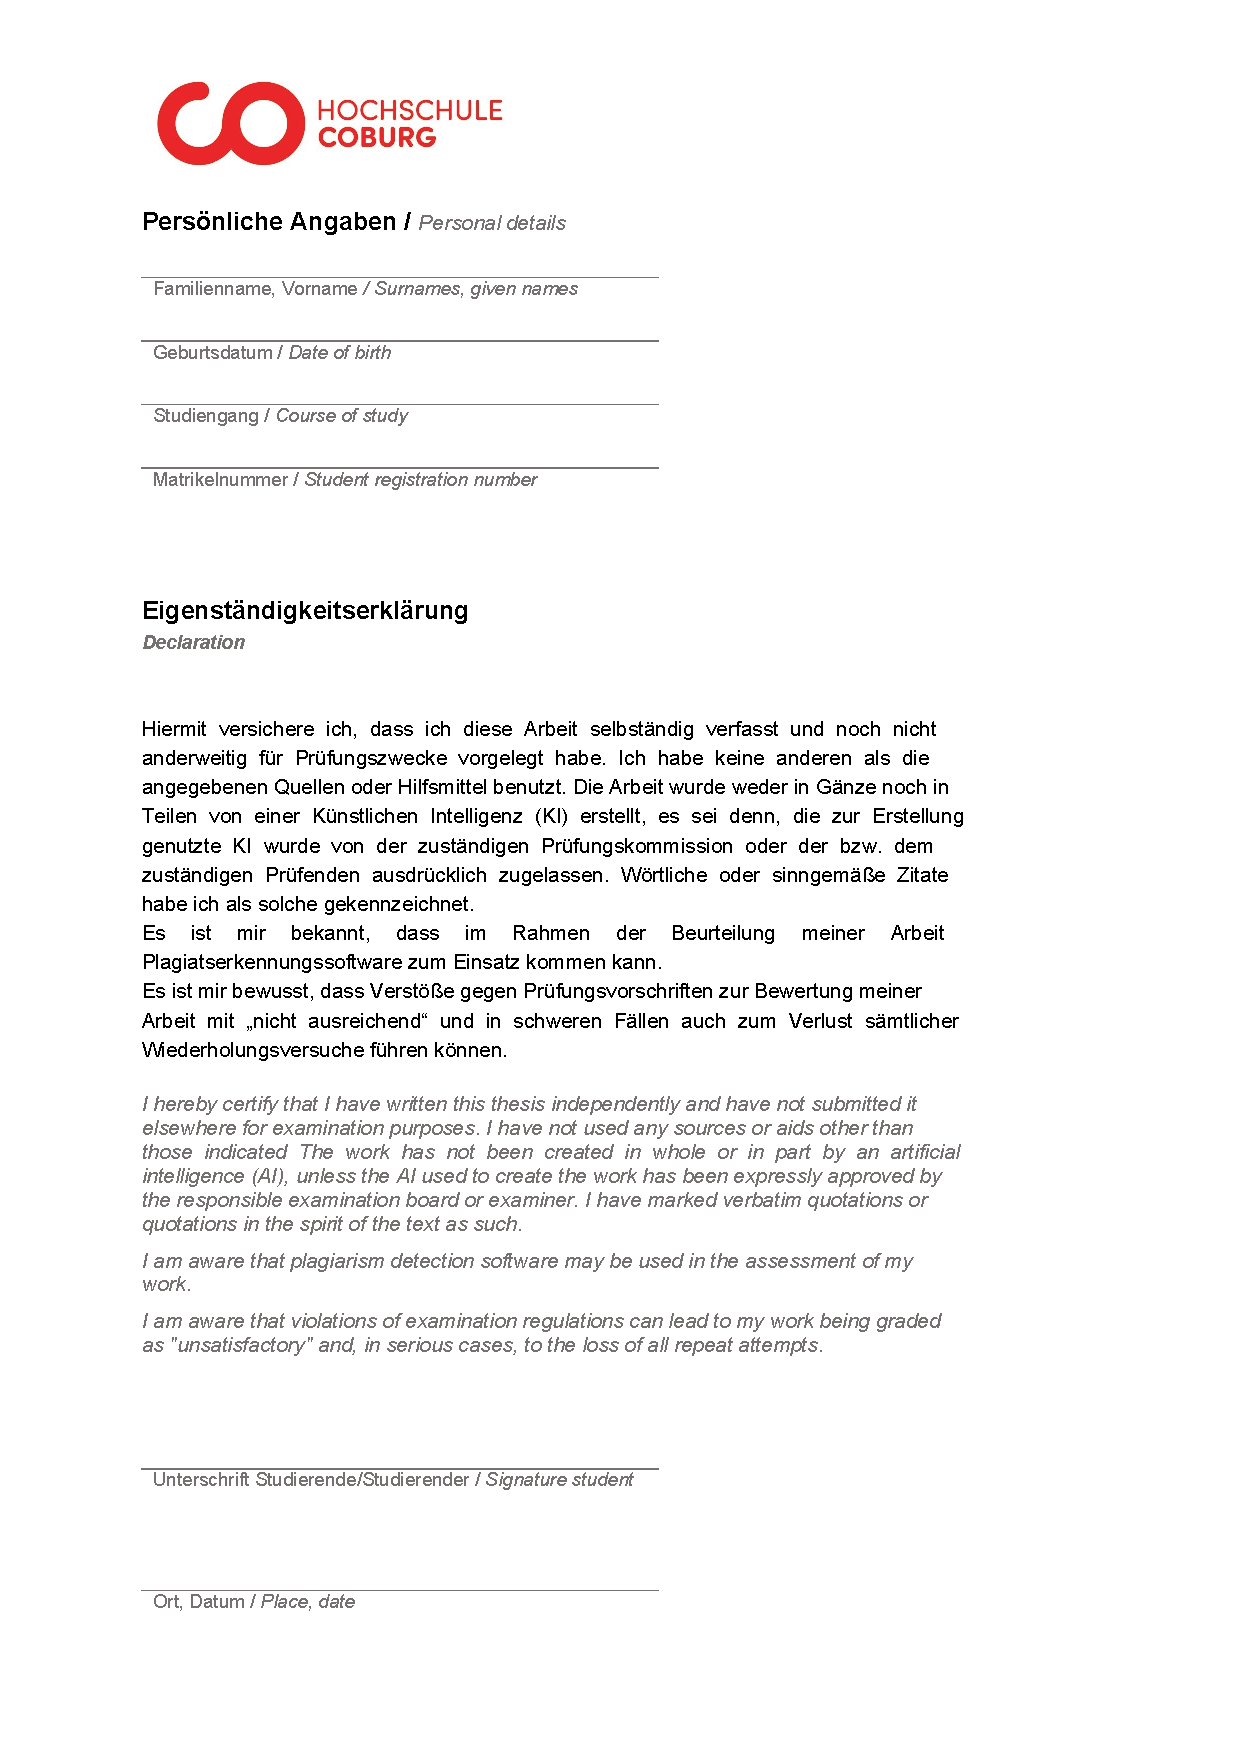
\includepdf[
  pages=-,
  pagecommand={},
  picturecommand*={
    \put(75,714){\large \Autorenname}
    \put(75,683){\large \Geburtsdatum}
    \put(75,652){\large \Studiengang}
    \put(75,622){\large \Matrikelnummer}
    \put(75,81.5){\large \Ort, den \today}
  }
]{framework/_Declaration_of_Honor.pdf}


  % TODO list
  \iftotalcounttodos
    \phantomsection
    \addcontentsline{toc}{section}{TODOs}
    \thispagestyle{empty}
    \listoftodos[TODOs]
  \fi
}

% ===========================================================================
%                   Simplified centered & colored tables
% ===========================================================================

\newenvironment{colortable}[1]{
  \begin{center}
    \begin{tabular}{#1}
    \hline
    \rowcolor{Gray}
}
{
    \hline
    \end{tabular}
  \end{center}
}

\newcommand{\tablecontent}{
  \hline
  \rowcolor{White}
}


\def\Titel{Vorlage für verschiedene Dokumente der HS Coburg}
\def\Dozent{<DOZENT>}

% Infos zum Autor
\def\Autorenname{<NACHNAME, VORNAME>}
\def\Geburtsdatum{<GEBURTSDATUM>}
\def\Matrikelnummer{<MATRIKELNUMMER>}
\def\Studiengang{<STUDIENGANG>}

% Infos zum Unternehmen
\def\Unternehmen{<FIRMENNAME>}
\def\Abteilung{<ABTEILUNG>}
\def\Strasse{<STRAßE>}
\def\Ort{<ORT>}

% Infos zum Betreuer
\def\Betreuer{<BETREUER>}
\def\Funktion{<FUNKTION BETREUER>}
\def\Telefon{<TELEFONNUMMER BETREUER>}
\def\Email{<BETREUER EMAIL>}

% Daten
\def\Beginn{<BEGINN>}
\def\Ende{<ENDE>}
\def\Abgabe{\today}

\begin{HSCDocument}[preset=Praxisbericht]

  \section{Einführung}
\label{sec:einfuehrung}

Bei diesem Dokument handelt es sich um eine \LaTeX{} Vorlage für wissenschaftliche Arbeiten in der \Acr{FEIF}. Es handelt sich hierbei nicht um eine Anleitung wie \LaTeX{} funktioniert, sondern rein um eine Vorlage die den formalen Richtlinien der \acr{FEIF} entspricht.

\newpage
\section{\LaTeX}

\LaTeX{} gehört zu den Typesetting-Sprachen und kann, einmal erlernt, die Schreibgeschwindigkeit
zum Verfassen wissenschaftlicher Arbeiten wesentlich erhöhen. Dies liegt vor allem daran, dass viele
manuelle Arbeitsschritte durch den \LaTeX{}-Compiler übernommen werden und somit automatisch ablaufen.

Nachfolgend wird ein kurzer Einblick in die Grundlagen von \LaTeX{} gegeben.

\subsection{Inhalt}

Das Inhaltsverzeichnis wird durch die Verwendung von Überschriften im Text automatisch erstellt.
Wird eine neue Überschrift hinzugefügt, taucht diese an der entsprechenden Stelle im Inhaltsverzeichnis auf.\\

Zudem gibt es noch weitere Verzeichnisse, die automatisch eingelayoutet werden.

\subsubsection{Abbildungen / Bilder}

Auch das Abbildungsverzeichnis wird automatisch erstellt. Hierzu muss eine Abbildung mit
entsprechender Syntax eingebunden werden. In diesem Beispiel wurde in Abbildung
\ref{fig: Lenna} das bekannte Standardtestbild für Bildbearbeitung "Lenna" eingebunden.

\begin{figure}[H]
  \centering
  
\includegraphics[width=.45\textwidth]{Lenna}
  \caption{Standard-Testbild für Bildbearbeitung "Lenna"}
  \label{fig: Lenna}
\end{figure}

Durch den "\textbackslash{}caption"-Befehl taucht die Grafik automatisch im Abbildungsverzeichnis auf.

\subsubsection{Tabellen}

Tabellen mit \LaTeX{} zu erstellen ist anfangs zugegebenermaßen etwas umständlich. Deswegen hier ein einfaches
Beispiel für eine Tabelle:

% Notiz: \hline erzeugt eine horizontale Linie

\begin{table}[H]
  \centering
  \begin{tabular}{|c|c|c|}
    \hline
    Spalte 1 & Spalte 2 & Spalte 3 \\
    \hline
    1.1 & 1.2 & 1.3 \\
    2.1 & 2.2 & 2.3 \\
    \hline
  \end{tabular}
  \caption{Beispieltabelle}
  \label{tab: Beispieltabelle}
\end{table}

Der "\textbackslash{}caption"-Befehl lässt die Tabelle wieder automatisch im Tabellenverzeichnis auftauchen.

\subsubsection{Codesnippets}

Codesnippets werden automatisch mit dem entsprechenden "Syntax Highlighting" angezeigt.
Hierbei lässt sich die Sprache pro Snippet ändern.
\vspace{.5cm}

\begin{lstlisting}[language=Python,caption=MD5-Hash-Generierung in Python]
import hashlib
password = '<PASSWORD>'
hashed = hashlib.md5((password + '5aM-2').encode()).hexdigest()
print(hashed)
\end{lstlisting}

\begin{lstlisting}[language=HTML,caption=HTML-Beispiel]
<body>
  <div class="example" id="test">
    <p>HTML Test</p>
  </div>
</body>
\end{lstlisting}

\subsection{Vorteile von \LaTeX}

\LaTeX{} macht es dem Autor besonders einfach, komplexe mathematische Formeln zu beschreiben, hier einige
Beispiele:

\begin{equation}
  \overline{x} = \frac{1}{n} \sum_{i=1}^n x_i
\end{equation}

\begin{align*}
  \int_0^2 x^2 &= 5 \\
  \lim_{x\to\infty} f(x) &= \sqrt{\ldots}
\end{align*}

Das Zitieren von verschiedenen Dokumenten ist in \LaTeX{} ebenso relativ einfach:

"Eine Faltung zweier Funktionen im Zeitbereich gestaltet sich als kompliziert, eine Vereinfachung
bringt es, die Funktionen in den Laplace-Bildbereich zu überführen.
Die Faltung im Zeitbereich entspricht einer Multiplikation im Bildbereich." \cite[S. 339f]{Papula2006}

Hierzu bietet es sich an, in einer genaueren Dokumentation zum Thema nachzulesen (Achtung: Englisch):
\url{https://www.overleaf.com/learn/latex/Bibliography_management_with_bibtex}

\section{Funktionalität}

Diese Vorlage wurde als Nachfolger der HS-internen Vorlage entworfen, welche aufgrund ihres
unmodularen Aufbaus nicht ohne Weiteres erweiterbar war. Zusätzlich sorgte auch die
Designentscheidung, "Boilerplate-Code" unabstrahiert in wesentliche Dateien (hauptsächlich Arbeit.tex)
zu integrieren, für unnötige Komplexität und visuelle Unordnung, was wiederum den Durchblick erschwerte.

Im Zuge der Überarbeitung wurden zahlreiche nicht benötigte Zeilen gelöscht und eine für
den Nutzer einfachere Umgebung geschaffen.

Verzeichnisse werden mit dieser Version nur eingefügt, wenn diese auch benötigt werden (siehe
\Gls{Glossar}). Sollten Packages fehlen oder Einstellungen hinzugefügt werden wollen,
so kann einfach eine Datei "Custom.tex" im gleichen Ordner wie "Arbeit.tex" erzeugt werden.
Diese Datei wird automatisch nach dem Laden der Vorlage ausgeführt und besitzt somit die
Möglichkeit, bereits gesetzte Werte und Variablen zu überschreiben.

Der Code wurde ausführlich kommentiert und sollte für den Autor ohne viel Mehraufwand veränderlich sein.

\subsection{Vorlagen-spezifische Funktionen}

Diese Vorlage stellt einige Funktionen zur Verfügung, die spezifisch für den Anwendungsfall sind.

\todo[inline,nolist,color=red!25,bordercolor=red]{!!! Die Definition des Templates liegt im Ordner "framework".
In diesem Ordner sollten keine Dateien gelöscht oder verändert werden.}

\subsubsection{Verwendung von Akronymen}

Bitte für Akronyme ausschließlich die unteren Kommandos benutzen, da das Abkürzungsverzeichnis
sonst nicht angezeigt wird.

\begin{itemize}
  \item \textbackslash{}acr\{xyz\} für Kurzform des Akronyms
  \item \textbackslash{}Acr\{xyz\} für die lange Form des Akronyms
\end{itemize}

\subsubsection{Symbolverzeichnis}

Über "\textbackslash{}nomen\{<ZEICHEN>\}\{<BESCHREIBUNG>\}" kann ein neuer Eintrag im
Symbolverzeichnis erzeugt werden. Die nachfolgenden Kommandos erleichtern die Erstellung
eines Eintrags, sind jedoch nicht zwangsläufig notwendig.

\begin{itemize}
  \item \textbackslash{}nomunit\{xyz\} für die rechte Spalte
  \item \textbackslash{}nomsi\{\textbackslash{}metre\} für die formatierte Einheit (hier Meter)
\end{itemize}

\subsubsection{Fortschrittsmanagement}

Beim Verfassen von Dokumenten auftauchende Ideen und Vorschläge können ohne Weiteres
im Text angemerkt werden, sodass diese in kommenden Änderungsdurchläufen berücksichtigt werden können.
Die sogenannten "TODOs" werden automatisch am Rand eingelayoutet.

\begin{itemize}
  \item \note{Beispielnotiz}\textbackslash{}note\{Beispielnotiz\} für eine neue Notiz am Rand
  \item \unsure{Überarbeitung anstehend}\textbackslash{}unsure\{Überarbeitung anstehend\}: eventuelle Überarbeitung später
  \item \change{Änderung}\textbackslash{}change\{Änderung\}: Änderungsidee
\end{itemize}

Sobald TODOs im Dokument vorhanden sind, werden diese ebenfalls auf der letzten Seite aufgeführt.

\subsubsection{Tabellen mit Kopfzeile}

Um Tabellen mit Kopfzeile einzufügen, kann die "\textbackslash{}colortable"-Umgebung genutzt werden.

\begin{table}[H]
  \centering

  % Custom tabular environment
  \begin{colortable}{|c|c|c|}
    Spalte 1 & Spalte 2 & Spalte 3 \\
    \tablecontent
    1.1 & 1.2 & 1.3 \\
    2.1 & 2.2 & 2.3 \\
  \end{colortable}

  \caption{Custom Tabelle}
  \label{tab: Tabelle 2}
\end{table}

\subsubsection{Referenzen}

Um Referenzen auf Abbildungen syntaktisch zu verkürzen, stellt das Template
ein eigenes Makro zur Verfügung: "\textbackslash{}imgref\{<LABEL>\}". Gleiches gilt
für Tabellen ("\textbackslash{}tabref\{<LABEL>\}").

Referenz auf Abbildung \ref{fig: Lenna}: \imgref{fig: Lenna}\\
Referenz auf Tabelle \ref{tab: Tabelle 2}: \tabref{tab: Tabelle 2}

\end{HSCDocument}
